
In this chapter we describe a canonical ladder for each $OptL\{\pi}\}$. We then provide a number of equations to calculate the 
location of the bar in the canonical ladder; depending on the configuration of $\pi$, we use different 
equations for calculating the location of the bar. We then define the data structure used to represent the canonical ladder. 
Using the data structure, we provide an algorithm for creating the canonical ladder for any $\pi$ of order $n$. Lastly, 
we describe the listing problem in relation to the canonical ladder. To see the canonical ladder for $(3,5,4,1,2)$, 
refer to Figure~\ref{Fig:Route}.
\begin{figure}[h]
	\centering
	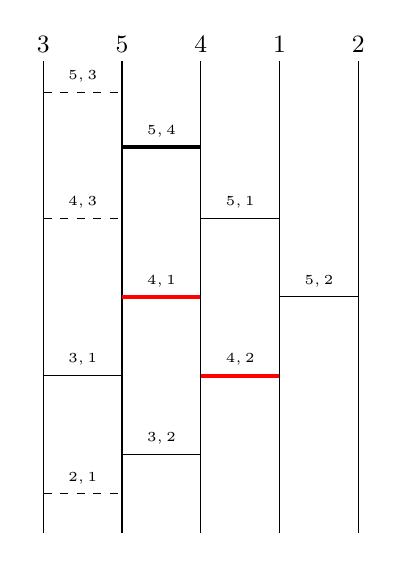
\begin{tikzpicture}
		\draw(0, 0) to (0, 6);
            \node at(.5, 5.8){\tiny{$5,3$}};
			\draw[dashed](0, 5.6) -- (1, 5.6);

            \node at(0.5, 4.2){\tiny{$4,3$}};
            \draw[dashed](0, 4) -- (1, 4);
			\node at(.5, 2.2){\tiny{$3,1$}};
			\draw(0, 2) to (1, 2);

            \draw[dashed](0, 0.5) -- (1, .5);
            \node at(.5, .7){\tiny{$2,1$}};
		\draw(1, 0) to (1, 6);
			\node at(1.5, 5.1){\tiny{$5,4$}};
			\draw[line width=.5mm](1, 4.9) to (2, 4.9);

			\node at(1.5, 3.2){\tiny{$4,1$}};
			\draw[line width=.5mm, red](1, 3.0) to (2, 3.0);

			\node at(1.5, 1.2){\tiny{$3,2$}};
			\draw(1, 1) to (2, 1);
	%		\node at(.75, .9){\tiny{$3,2$}};
	%		\draw(.5, .7) to (1, .7);
		\draw(2, 0) to (2, 6);

			\node at(2.5, 4.2){\tiny{$5,1$}};
			\draw(2, 4) to (3, 4);


			\node at(2.5, 2.2){\tiny{$4,2$}};
			\draw[line width=.5mm, red](2, 2) to (3, 2);
			%\node at(1.25, 2.1){\tiny{$4,1$}};
			%\draw[line width=.5mm, red ](1, 1.9) to (1.5, 1.9);
			%\node at(1.25, 1.3){\tiny{$5,2$}};
			%\draw(1, 1.1) to(1.5, 1.1);
		\draw(3, 0) to (3, 6);
			
			\node at(3.5, 3.2){\tiny{$5,2$}};
			\draw(3, 3.0) to (4, 3.0);	
		%\node at(1.75, 1.7){\tiny{$4,2$}};
			%\draw[line width=.5mm, red ](1.5, 1.5) to (2, 1.5);
			%\node at(1.75, .9){\tiny{$5,4$}};
			%\draw[line width=.5mm, red ](1.5, .7) to (2, .7);
		\draw(4, 0) to (4, 6);


		\node at(0.0, 6.2){\small{$3$}};
		\node at(1, 6.2){\small{$5$}};
		\node at(2.0, 6.2){\small{$4$}};
		\node at(3, 6.2){\small{$1$}};
		\node at(4, 6.2){\small{$2$}};
	\end{tikzpicture}
	\caption{The canonical ladder for $(3,5,4,1,2)$. Bars $(5,4),(4,1),(4,2)$ are part of the route of 
    $4$, but only the red bars are associated with the route of $4$.}
	\label{Fig:Route}
\end{figure}


\section{The Canonical Ladder in Detail}
In this section, we fully define the canonical ladder corresponding to $\pi$. We first define the associated terminology in order 
to provide a comprehensive definition of the canonical ladder.
Let the \emph{route} of an element be the sequence of bars the element travels along in order to reach its final position in the 
sorted permutation. The bars are read from top to bottom. In Figure~\ref{Fig:Route}, the bars $(5,4),(4,1)$ and $(4,2)$ compose the route of $4$. 
For every bar, two elements cross the bar, therefore \emph{bar association} is the association of a bar with the greater of the two elements that 
cross it. For example, in Figure~\ref{Fig:Route}, element $4$ has the bars $(5,4),(4,1)$ and 
$(4,2)$ in its route, however only bars $(4,1)$ and $(4,2)$ are associated with element $4$. Let the \emph{absence of a bar} corresponding to 
two uninverted elements in $\pi$, $x>y$, be defined as a dashed, horizontal line spanning across a column in the ladder. 
We say \emph{absence of a bar association} is the association of the absence of a bar with the greater of the two elements that form it. 
For example,$(5,3)$ are uninverted in $(3,5,4,1,2)$, therefore the absence of the bar is associated with $5$. 
For each element $2 \leq x \leq n \in \pi$, we define the \emph{associated diagonal of x} as a diagonal with $x-1$ 
row and column coordinates, having one endpoint at $(2n-2x+1, 1)$ and the other endpoint at $(2n-x-1,x-1)$.  
At each row and column in the associated diagonal of $x$, either a bar associated with $x$ or the absence of a bar associated with $x$ exists. 
For an example of the associated diagonals for the ladder corresponding to $(3,4,2,1,5)$ refer to Figure~\ref{fig:my_label}. 
\begin{figure}[h]
    \centering
    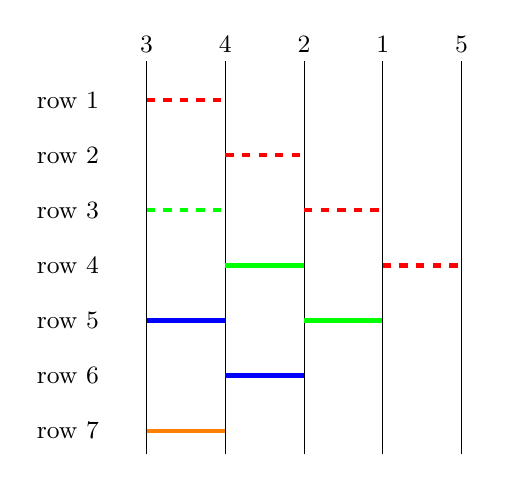
\begin{tikzpicture}
        \draw(0,0) to (0,5);
            \draw[red, dashed, line width=0.55mm](0, 4.5) -- (1,4.5);
            \draw[green, dashed, line width=0.55mm](0, 3.1) -- (1,3.1);
            \draw[blue, line width=0.55mm](0, 1.7) to (1,1.7);
            \draw[orange, line width=0.55mm](0, 0.3) to (1,0.3);

        \draw(1,0) to (1,5);
            \draw[red, dashed, line width=0.55mm](1, 3.8) -- (2,3.8);
            \draw[green, line width=0.55mm](1, 2.4) to (2,2.4);
            \draw[blue, line width=0.55mm](1, 1.0) to (2,1.0);
        \draw(2,0) to (2,5);
           \draw[red, dashed, line width=0.55mm](2, 3.1) -- (3,3.1);
            \draw[green, line width=0.55mm](2, 1.7) to (3,1.7);
        \draw(3,0) to (3,5);
         \draw[red, dashed, line width=0.55mm](3, 2.4) -- (4,2.4);
        \draw(4,0) to (4,5);

        \node at (-1, 4.5){\small{row 1}};
        \node at (-1, 3.8){\small{row 2}};
        \node at (-1, 3.1){\small{row 3}};
        \node at (-1, 2.4){\small{row 4}};
        \node at (-1, 1.7){\small{row 5}};
        \node at (-1, 1.0){\small{row 6}};
        \node at (-1, 0.3){\small{row 7}};

        \node at(0, 5.2){\small{$3$}};
        \node at(1, 5.2){\small{$4$}};
        \node at(2, 5.2){\small{$2$}};
        \node at(3, 5.2){\small{$1$}};
        \node at(4, 5.2){\small{$5$}};

    \end{tikzpicture}
    \caption{The associated diagonal of $5$ is in red, the associated diagonal of $4$ is in green, the associated diagonal of $3$ is in blue, and the associated diagonal of $2$ is in orange.}
    \label{fig:my_label}
\end{figure}

With the definition of the associated diagonal, we are now able to fully define the \emph{canonical ladder} as 
the ladder such that for each element $2 \leq x \leq n$, each bar, and absence of a bar, associated with $x$ exists 
along the associated diagonal of $x$. %Given $\pi$, we construct $CL(\pi)$ by using equation~\ref{getCordEqn} found in section 
%\textbf{Calculating the Location of a Bar for an Arbitrary $CL(\pi_{n})$}, 
%and Algorithm~\ref{Alg:RootLadder} found in section \textbf{Algorithm: Create Canonical}. 
We note that the two aforementioned figures, Figure~\ref{Fig:Route} and Figure~\ref{fig:my_label}, are the canonical ladders 
corresponding to each of their respective permutations. We use $CL(\pi)$ as shorthand notation for `the canonical ladder corresponding 
to a permutation of order $n$'. 

\section{Locating the Bar for a Given Inversion in an Arbitrary $CL(\pi)$}
In this section, we provide an equation for locating the bar in the canonical ladder associated with a given inversion, 
in an arbitrary permutation 
of order $n$. As previously stated, every bar associated with some element $x$ exists along the associated diagonal of $x$ 
within the canonical ladder. 
We use Equation~\ref{getCordEqn}, to determine the row and column for the bar corresponding 
to two elements, $x>y$, along the associated diagonal of $x$. 
Let $\pi$ be an arbitrary permutation of order $n$. Let 
$pos(x)$ be the index of $x \in \pi$. To calculate the row and column of the bar, or absence of a bar, for a pair of elements 
$x>y$, we first map $x$ to a new index termed $pos'(x)$. Let $pos'(x)$ equal $pos(x)$ minus the number of elements greater than $x$ and 
 to the left of $x$ in $\pi$. 
For example, given $\pi=(3,2,7,4,8,5,6,9,1)$, 
suppose $x=6$, then $pos'(6)=pos(6)-2=5$. 
Once we have calculated $pos'(x)$ we use a similar method to calculate $pos'(y)$. $pos'(y)$ equals 
$pos(y)$ minus the number of elements greater than $y$ and to the left of $y$ excluding $x$. For example, suppose $x$ is $7$ and 
$y$ is $5$, then $pos'(y)$ is $pos(y)-1=5$. Once we have $pos'(x)$ and $pos'(y)$, we use Equation~\ref{getCordEqn} 
to return the row and column for the bar, or absence of the bar,  
along the associated diagonal of $x$.
\begin{equation}\label{getCordEqn}
\resizebox{.9\textwidth}{!}{
\[   
    (row,column)=
    \begin{cases}
        ((2n - x - 1) - (x - pos'(y))+1,(x-1)-(x-pos'(y))+1) & \text{if $pos'(x)>pos'(y)$} \\ 
        ((2n - x - 1) - (x-pos'(y)), (x-1) - (x-pos'(y)) & \text{if $pos'(y)>pos'(x)$}
    \end{cases}
\]
}
\end{equation}

Given the inversion $(7,5) \in (3,2,7,4,8,5,6,9,1)$, we calculate the row and column of the bar $(7,5)$ using the second case. We 
get $row=(18 - 7 - 1) - (7 - 5)=8$ and $col=6-(7-5)=4$. To calculate $pos'(x)$ and $pos'(y)$, is linear amortized time. Once $pos'(x)$ 
and $pos'(y)$ are calculated,  returns the location in $O(1)$ time. 
We can use Equation~\ref{getCordEqn} to look up the location of any bar for a given $\pi$. 
In Figure~\ref{Fig:CanLArbitrary} we see $CL(3,2,7,4,8,5,6,9,1)$, where each row and column is calculated using Equation~\ref{getCordEqn}. 
\pagebreak
\begin{figure}[t]
    \centering
    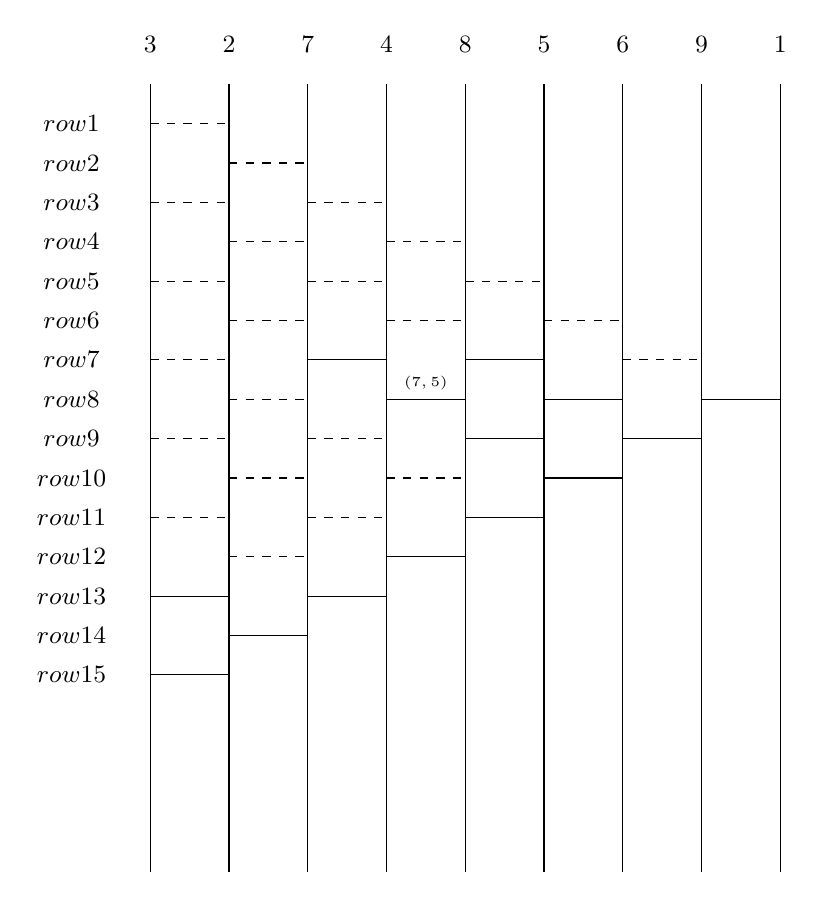
\begin{tikzpicture}
        \draw(0,0) to (0,10);
            \draw[dashed] (0, 9.5) -- (1, 9.5);
            \draw[dashed] (0, 8.5) -- (1, 8.5);
            \draw[dashed] (0, 7.5) -- (1, 7.5);
            \draw[dashed] (0, 6.5) -- (1, 6.5);
            \draw[dashed]         (0, 5.5) -- (1, 5.5);
            \draw[dashed]         (0, 4.5) -- (1, 4.5);
            \draw         (0, 3.5) to (1, 3.5);
            \draw         (0, 2.5) to (1, 2.5);
        \draw(1,0) to(1,10);
            \draw[dashed] (1, 9) -- (2, 9);
            \draw[dashed] (1, 8) -- (2, 8);
            \draw[dashed] (1, 7) -- (2, 7);
                
            \draw[dashed] (1, 6) -- (2, 6);
            \draw[dashed] (1, 5) -- (2, 5);
            \draw[dashed] (1, 4) -- (2, 4);
            \draw (1, 3) to (2, 3);
        \draw(2,0) to(2,10);
            \draw[dashed] (2, 8.5) -- (3, 8.5);
            \draw[dashed] (2, 7.5) -- (3, 7.5);
            \draw         (2, 6.5) to (3, 6.5);
            \draw[dashed] (2, 5.5) -- (3, 5.5);
            \draw[dashed] (2, 4.5) -- (3, 4.5);
            \draw         (2, 3.5) to (3, 3.5);
        \draw(3,0) to(3,10);
            \draw[dashed](3, 8) -- (4, 8);
            \draw[dashed](3, 7) -- (4, 7);
            \node at(3.5, 6.2){\tiny{$(7,5)$}};
            \draw        (3, 6) to (4, 6);
            \draw[dashed](3, 5) -- (4, 5);
            \draw        (3, 4) to (4, 4);
        \draw(4,0) to(4,10);
            \draw[dashed](4, 7.5) -- (5, 7.5);
            \draw(4, 6.5) to (5, 6.5);
            \draw(4, 5.5) to (5, 5.5);
            \draw(4, 4.5) to (5, 4.5);
        \draw(5,0) to(5,10);
            \draw[dashed](5, 7) -- (6, 7);
            \draw(5, 6) to (6, 6);
            \draw(5, 5) to (6, 5);
        \draw(6,0) to(6,10);
            \draw[dashed](6, 6.5) to (7, 6.5);
            \draw        (6, 5.5) to (7, 5.5);
        \draw(7,0) to(7,10);
            \draw(7, 6) to (8, 6);
        \draw(8,0) to(8,10);

        \node at(0, 10.5){\small{$3$}};
        \node at(1, 10.5){\small{$2$}};
        \node at(2, 10.5){\small{$7$}};
        \node at(3, 10.5){\small{$4$}};
        \node at(4, 10.5){\small{$8$}};
        \node at(5, 10.5){\small{$5$}};
        \node at(6, 10.5){\small{$6$}};
        \node at(7, 10.5){\small{$9$}};
        \node at(8, 10.5){\small{$1$}};

        \node at(-1, 9.5){\small{$row 1$}};
        \node at(-1, 9.0){\small{$row 2$}};
        \node at(-1, 8.5){\small{$row 3$}};
        \node at(-1, 8.0){\small{$row 4$}};
        \node at(-1, 7.5){\small{$row 5$}};
        \node at(-1, 7.0){\small{$row 6$}};
        \node at(-1, 6.5){\small{$row 7$}};
        \node at(-1, 6.0){\small{$row 8$}};
        \node at(-1, 5.5){\small{$row 9$}};
        \node at(-1, 5.0){\small{$row 10$}};
        \node at(-1, 4.5){\small{$row 11$}};
        \node at(-1, 4.0){\small{$row 12$}};
        \node at(-1, 3.5){\small{$row 13$}};
        \node at(-1, 3.0){\small{$row 14$}};
        \node at(-1, 2.5){\small{$row 15$}};
    \end{tikzpicture}
    \caption{Canonical ladder such that each bar or absence of a bar is calculated using the Equation~\ref{getCordEqn}.}
    \label{Fig:CanLArbitrary}
\end{figure}




\section{Locating the Bar for a Given Inversion in $CL((n,n-1, \dots 1))$}
In the previous section, we looked up a bar for a given inversion for some arbitrary permutation 
in $O(n)$ time. Clearly this is less than ideal. However, if $\pi$ is an arbitrary permutation 
of order $n$, we require linear time to calculate the location of a bar. 
In this section, we calculate the location of a bar corresponding to an inversion for $CL((n,n-1, \dots, 1))$ 
in $O(1)$ time. 
Let  $\pi=(n,n-1,n-2,...,1)$, then each associated diagonal in $CL(\pi)$ is fully occupied by bars. 
Let $x,y$ be a pair of elements in $\pi$ such that $x>y$ and $2 \leq x \leq n$. 
We know there exists a bar, $(x,y)$, in $CL((n,n-1, \dots 1))$ along the associated diagonal of $x$.
We compute the row and column of a bar $(x,y)$ in $CL((n,n-1, \dots 1))$ in $O(1)$ time using Equation~\ref{revCordEqn}. 
\begin{equation} \label{revCordEqn}
(row,column)=(2n-2x + (x-y), (x-y))
\caption{GetCoordinatesReverse}
\end{equation}

For example, given $\pi=(6,5,4,3,2,1)$, bar $(5,2)$ is located at row $5$; note that $5=(2n-2x)+(x-y)$. Bar $(5,2)$ is also located at column 
$3$; note that $3=x-y$. To see the canonical ladder for $(6,5,4,3,2,1)$ with the corresponding 
bars, please refer to Figure~\ref{Fig:RootLadderReverse}.
\begin{figure}[h]
    \centering
    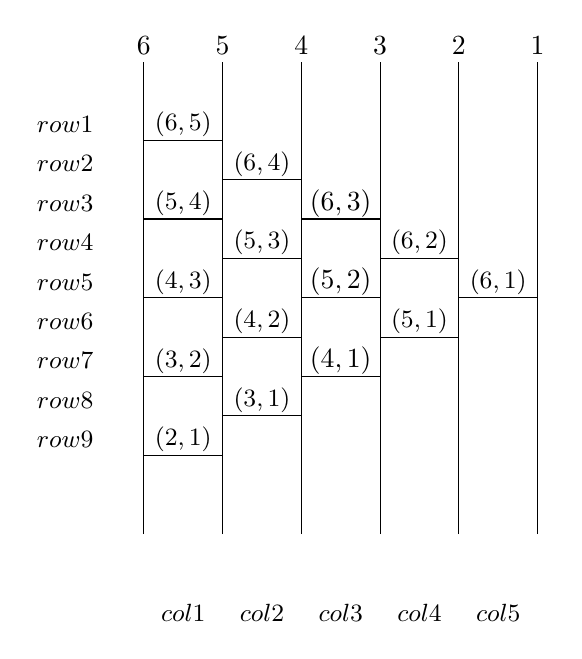
\begin{tikzpicture}
        \draw(0,0) to (0,6);
            \node at (0.5, 5.2){\small{$(6,5)$}};
            \draw(0, 5) to (1, 5);
            \node at (0.5, 4.2){\small{$(5,4)$}};
            \draw(0, 4) to (1, 4);
            \node at (0.5, 3.2){\small{$(4,3)$}};
            \draw(0, 3) to (1, 3);
            \node at (0.5, 2.2){\small{$(3,2)$}};
            \draw(0, 2) to (1, 2);
            \node at (0.5, 1.2){\small{$(2,1)$}};
            \draw(0, 1) to (1, 1);
        \draw(1,0) to (1,6);
            \node at(1.5, 4.7){\small{$(6,4)$}};
            \draw(1, 4.5) to (2, 4.5);
            \node at(1.5, 3.7){\small{$(5,3)$}};
            \draw(1, 3.5) to (2, 3.5);
            \node at(1.5, 2.7){\small{$(4,2)$}};
            \draw(1, 2.5) to (2, 2.5);
            \node at(1.5, 1.7){\small{$(3,1)$}};
            \draw(1, 1.5) to (2, 1.5);
        \draw(2,0) to (2,6);
            \node at(2.5, 4.2){$(6,3)$};
            \draw(2, 4) to (3, 4);
            \node at(2.5, 3.2){$(5,2)$};
            \draw(2, 3) to (3, 3);
            \node at(2.5, 2.2){$(4,1)$};
            \draw(2, 2) to (3, 2);
        \draw(3,0) to (3,6);
            \node at(3.5, 3.7){\small{$(6, 2)$}};
            \draw(3, 3.5) to (4, 3.5);
            \node at(3.5, 2.7){\small{$(5, 1)$}};
            \draw(3, 2.5) to (4, 2.5);
        \draw(4,0) to (4,6);
            \node at(4.5, 3.2){\small{$(6,1)$}};
            \draw(4, 3) to (5, 3);
        \draw(5,0) to (5,6);

        \node at(0, 6.2){$6$};
        \node at(1, 6.2){$5$};
        \node at(2, 6.2){$4$};
        \node at(3, 6.2){$3$};
        \node at(4, 6.2){$2$};
        \node at(5, 6.2){$1$};

        \node at(-1, 5.2){\small{$row 1$}};
        \node at(-1, 4.7){\small{$row 2$}};
        \node at(-1, 4.2){\small{$row 3$}};
        \node at(-1, 3.7){\small{$row 4$}};
        \node at(-1, 3.2){\small{$row 5$}};
        \node at(-1, 2.7){\small{$row 6$}};
        \node at(-1, 2.2){\small{$row 7$}};
        \node at(-1, 1.7){\small{$row 8$}};
        \node at(-1, 1.2){\small{$row 9$}};

        \node at(0.5, -1){\small{$col1$}};
        \node at(1.5, -1){\small{$col2$}};
        \node at(2.5, -1){\small{$col3$}};
        \node at(3.5, -1){\small{$col4$}};
        \node at(4.5, -1){\small{$col5$}};
    \end{tikzpicture}
    \caption{Canonical ladder for $(6,5,4,3,2,1)$. The location of each bar can be calculated using the formula $(2n-2x + (x-y), (x-y))$}
    \label{Fig:RootLadderReverse}
\end{figure}
We use Equation~\ref{revCordEqn} to locate a bar when we know $\pi=(n,n-1, \dots, 2,1)$. We use Equation~\ref{revCordEqn} when possible 
because the calculation time is $O(1)$ rather than $O(n)$. 


% in the corresponding $CL(\pi_{n})$. Further work is required to determine if removing bars from $CL(n,n-1, \dots, 1)$ 


\section{Algorithm: {\sc CreateCanonical}}
In this section we provide the data structure used to represent the canonical ladder in code. We then provide the algorithm for creating the canonical ladder corresponding to any permutation of 
order $n$. 
To create the canonical ladder 
we must represent the canonical ladder in code. We use Theorem~\ref{Theorem:RootHeight} and Corollary~\ref{Corollary:RootHeight} to prove the 
veracity of the representation of the canonical ladder.
 \begin{theorem}
   The number of rows required for the canonical ladder corresponding to the descending permutation of order $n$ is $2(n-1) - 1$.
   \label{Theorem:RootHeight}
 \end{theorem}
 \begin{proof}
 	Let $\pi$ be the descending permutation of order $n$. Let $route(x)$ be the route of $n \geq x \geq 2 \in \pi$. We know that 
     when $x=n$, $route(x)$ has $n-1$ bars, each requiring their own row. Thus, $CL((n,n-1, \dots, 1))$ requires at least $n-1$ rows. 
     For each subsequent $x$ from $[n-1 \dots 2]$, each $route(x)$ requires one more row to be added to $CL((n, n-1, \dots 1))$. 
     We get an additional $n-2$ rows added to $CL$, one for each $route([n-1 \geq x \geq 2])$. Therefore, the total number of rows is 
     $(n-1)+(n-2)=2(n-1)-1$.
 \end{proof}

 \begin{corollary}
     The upper bound for the number of rows of any canonical ladder of order $n$ is $2(n-1)-1$.
     \label{Corollary:RootHeight}
 \end{corollary}
 \begin{proof}
     By Theorem~\ref{Theorem:RootHeight}, we know that $2(n-1)-1$ is the number of rows required for 
     the canonical ladder corresponding 
     to the descending permutation of order $n$. By removing 
     bars from the canonical ladder for the descending permutation of order $n$, we can derive any other canonical ladder for any other permutation 
     of order $n$; removing a bar translates to removing an 
     inversion in $\pi$. Removing bars from the canonical ladder corresponding to the descending permutation of order $n$ 
     does not necessarily remove a row from the ladder, however, removing bars from the ladder certainly does not add any more rows 
     to $ladder$. Therefore, $2(n-1)-1$ is the upper bound for the number of rows required for any ladder of order $n$.
 \end{proof}
Using Theorem~\ref{Theorem:RootHeight} and Corollary~\ref{Corollary:RootHeight}, 
we represent a canonical ladder as a binary matrix with $2(n-1)-1$ rows and $n-1$ columns. Let $matrix[row][col]=1$ 
indicate a bar at the given row and column in the canonical ladder along an associated diagonal. Let $matrix[row][col]=0$ indicate the absence 
of a bar at the given row and column in the canonical ladder along an associated diagonal. Let $matrix[row][col]=-$ indicate irrelevancy as to whether 
a $1$ or $0$ is at the given row and column because the row and column do not lie on an associated diagonal. To see the canonical ladder for 
$(4,2,1,3)$ and the corresponding binary matrix, refer to Figure~\ref{Fig:MatrixLadder}.
\begin{figure}[ht]
    \begin{minipage}{.4\textwidth}
        \centering
        \begin{tikzpicture}
        \node at(0, 4.2){\small{$4$}};
        \node at(1, 4.2){\small{$2$}};
        \node at(2, 4.2){\small{$1$}};
        \node at(3, 4.2){\small{$3$}};
        \draw(0, 0) to (0, 4);
            \draw(0,3.9) to (1,3.9);
            \draw[dashed](0,1.9) -- (1,1.9);
            \draw(0,0.1) to (1,0.1);
        \draw(1, 0) to (1, 4);
            \draw(1,2.9) to (2,2.9);
            \draw[dashed](1,0.9) -- (2,0.9);
        \draw(2, 0) to (2, 4);
            \draw(2,1.9) to (3,1.9);
        \draw(3, 0) to (3, 4);
        \end{tikzpicture}
    \end{minipage}
    \begin{minipage}{0.4\textwidth}
        \begin{flushright}
        \begin{bmatrix}
            1 & - & - \\
            - & 1 & -\\
            0 & - & 1 \\ 
            - & 0 & - \\
            1 & - & - \\

        \end{bmatrix}
    \end{flushright}
    \end{minipage}
    \caption{Canonical ladder and corresponding binary matrix.}
    \label{Fig:MatrixLadder}
\end{figure}

Using Equation~\ref{getCordEqn}, and the binary matrix representation 
of a ladder, we define algorithm {\sc CreateCanonical} which can be found 
in Algorithm~\ref{Alg:RootLadder} to create the canonical ladder for 
any given permutation of order $n$. 
The initial conditions of {\sc CreateCanonical} are the 
following. Let $ladder$ be the binary matrix representing $CL(\pi)$ initialized to $-$. Let $\pi$ be an arbitrary permutation 
of order $n$. Let $x$ be the currently maximal element in $\pi$, initialized to $n$. Let {\sc GetCoordinates} refer to 
Equation~\ref{getCordEqn}. 
\begin{algorithm}[ht]
	\begin{algorithmic}[1]
		\Function {CreateCanonical}{$ladder$, $\pi$, $x$}
			\While{$x>1$}
                \State $pos(x) \gets $ index of $x \in \pi$
                \For{$i$ \textbf{from} $1$  \textbf{to} $x$}
                    \If{$i \neq pos(x)$}
                        
                        \State $(row, column) \gets${\sc GetCoordinates($x$, $pos(x), i$)}
                        \If{$pos(x)<i$}
                            \State $ladder[row][col] \gets 1$
                        \Else
                            \State $ladder[row][col] \gets 0$
                        \EndIf
                    \EndIf
                \EndFor
                \State $\pi \gets \pi - x$
                \State $x \gets x-1$
            \EndWhile
        \EndFunction

	\end{algorithmic}
	\caption{The algorithm for creating the canonical ladder of $OptL\{\pi\}$}
	\label{Alg:RootLadder}
\end{algorithm}

On each iteration of the while loop, all $x-1$ $1s$ and $0s$  along the associated diagonal of the $xth$ 
element are added to $ladder$ within the for-loop. {\sc GetCoordinates}, which refers to Equation~\ref{getCordEqn}, 
returns the row and column coordinate for the respective $1$ or $0$ for the pair of elements, $x>y$. Note that we call {\sc GetCoordinates} with 
the arguments $(x,pos(x),i)$. When referring to Equation~\ref{getCordEqn} the variables 
are $(x,pos'(x),pos'(y))$. Prior to the next iteration of the while loop, 
$x$ is removed from $\pi$ and all elements to the right of $x$ are moved to the left by one index. 
Then, $x$ is decremented by $1$. The while loop continues until $x=1$. Determining $pos(x)$ 
is done in $O(x)$ time. Removing $x$ from $\pi$ is done in $O(x)$ time. Calculating the row and column 
for each $(x,y)$ is done in $O(1)$ time. Overall, the algorithms complexity is $O(n^2)$.
We also note that {\sc CreateCanonical} creates the ladder representation with clean level $1$.  
Given three elements, $x>y>z$ and $pos(x) < pos(y) < pos(z)$, Equation~\ref{getCordEqn} returns a lesser row 
for $(x,z)$ than for $(y,z)$. Therefore, {\sc CreateCanonical} creates a representation of a ladder with clean level $1$. 
To see the resulting state of the ladder for each iteration of {\sc CreateCanonical} with $(5,7,3,4,1,2,6)$ please refer to Figure~\ref{Fig:CreateRoot}. 
\begin{figure}[t]
    \centering 
    \begin{minipage}{.3\textwidth}
    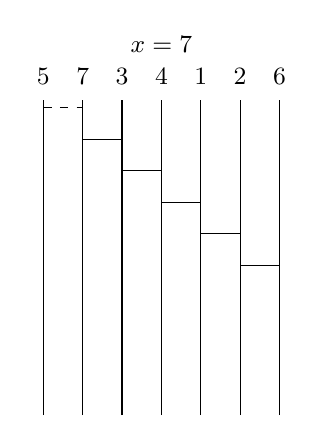
\begin{tikzpicture}
        \draw(0, 0) to (0, 4);
        
        \draw(.5, 0) to (.5, 4);
        \draw(1, 0) to (1, 4);
        \draw(1.5, 0) to (1.5, 4);
        \draw(2, 0) to (2, 4);
        \draw(2.5, 0) to (2.5, 4);
        \draw(3, 0) to (3, 4);
        
        \draw(2.5, 1.9) to (3, 1.9);
        \draw(2.0, 2.3) to (2.5, 2.3);
        \draw(1.5, 2.7) to (2.0, 2.7);
        \draw(1.0, 3.1) to (1.5, 3.1);
        \draw(0.5, 3.5) to (1.0, 3.5);

        \draw[dashed] (0, 3.9) -- (0.5, 3.9);
        \node at(1.5, 4.7){\small{$x=7$}};
        \node at(0, 4.3){\small{$5$}};
        \node at(.5, 4.3){\small{$7$}};
        \node at(1, 4.3){\small{$3$}};
        \node at(1.5, 4.3){\small{$4$}};
        \node at(2, 4.3){\small{$1$}};
        \node at(2.5, 4.3){\small{$2$}};
        \node at(3, 4.3){\small{$6$}};
    \end{tikzpicture}
    \end{minipage}
    \begin{minipage}{.3\textwidth}
    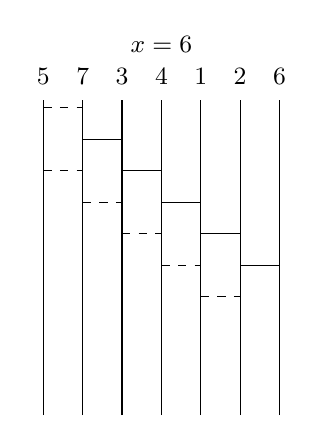
\begin{tikzpicture}
        \draw(0, 0) to (0, 4);
        \draw(.5, 0) to (.5, 4);
        \draw(1, 0) to (1, 4);
        \draw(1.5, 0) to (1.5, 4);
        \draw(2, 0) to (2, 4);
        \draw(2.5, 0) to (2.5, 4);
        \draw(3, 0) to (3, 4);
        
        \draw[dashed] (0, 3.9) -- (0.5, 3.9);
        \draw[dashed] (2, 1.5) -- (2.5, 1.5);
        \draw[dashed] (1.5, 1.9) -- (2.0, 1.9);
        \draw[dashed] (1.0, 2.3) -- (1.5, 2.3);
        \draw[dashed] (0.5, 2.7) -- (1.0, 2.7);
        \draw[dashed] (0.0, 3.1) -- (0.5, 3.1);
        \draw(2.5, 1.9) to (3, 1.9);
        \draw(2.0, 2.3) to (2.5, 2.3);
        \draw(1.5, 2.7) to (2.0, 2.7);
        \draw(1.0, 3.1) to (1.5, 3.1);
        \draw(0.5, 3.5) to (1.0, 3.5);

        \node at(1.5, 4.7){\small{$x=6$}};

        \node at(0, 4.3){\small{$5$}};
        \node at(.5, 4.3){\small{$7$}};
        \node at(1, 4.3){\small{$3$}};
        \node at(1.5, 4.3){\small{$4$}};
        \node at(2, 4.3){\small{$1$}};
        \node at(2.5, 4.3){\small{$2$}};
        \node at(3, 4.3){\small{$6$}};
    \end{tikzpicture}
    \end{minipage}
   \begin{minipage}{.3\textwidth}
    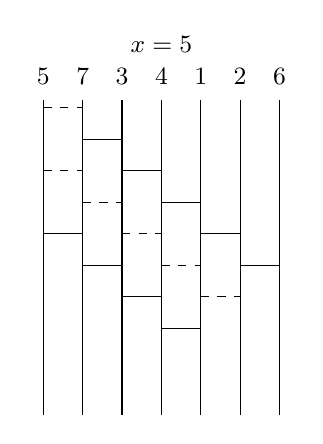
\begin{tikzpicture}
        \draw(0, 0) to (0, 4);
            \draw(0, 2.3) to (0.5, 2.3);
        \draw(.5, 0) to (.5, 4);
            \draw(.5, 1.9) to (1, 1.9);
        \draw(1, 0) to (1, 4);
            \draw(1, 1.5) to (1.5, 1.5);
        \draw(1.5, 0) to (1.5, 4);
            \draw(1.5, 1.1) to (2, 1.1);
            \draw(1.5, 2.7) to (2, 2.7);
        \draw(2, 0) to (2, 4);
        \draw(2.5, 0) to (2.5, 4);
        \draw(3, 0) to (3, 4);
      


        \draw(2.5, 1.9) to (3, 1.9);
        \draw(2.0, 2.3) to (2.5, 2.3);

        \draw(1.0, 3.1) to (1.5, 3.1);
        \draw(0.5, 3.5) to (1.0, 3.5);
      
        \draw[dashed] (0, 3.9) -- (0.5, 3.9);
        \draw[dashed] (2, 1.5) -- (2.5, 1.5);
        \draw[dashed] (1.5, 1.9) -- (2.0, 1.9);
        \draw[dashed] (1.0, 2.3) -- (1.5, 2.3);
        \draw[dashed] (0.5, 2.7) -- (1.0, 2.7);
        \draw[dashed] (0.0, 3.1) -- (0.5, 3.1);
        

        \node at(1.5, 4.7){\small{$x=5$}};
        \node at(0, 4.3){\small{$5$}};
        \node at(.5, 4.3){\small{$7$}};
        \node at(1, 4.3){\small{$3$}};
        \node at(1.5, 4.3){\small{$4$}};
        \node at(2, 4.3){\small{$1$}};
        \node at(2.5, 4.3){\small{$2$}};
        \node at(3, 4.3){\small{$6$}};
    \end{tikzpicture}
    \end{minipage}
        
    \begin{minipage}{.3\textwidth}
    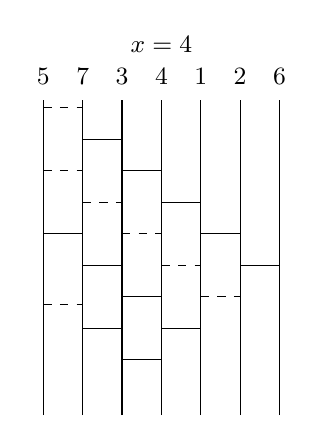
\begin{tikzpicture}
    \draw(0, 0) to (0, 4);
            \draw(0, 2.3) to (0.5, 2.3);
        \draw(.5, 0) to (.5, 4);
            \draw(.5, 1.9) to (1, 1.9);
            \draw(0.5, 1.1) to (1, 1.1);
        \draw(1, 0) to (1, 4);
            \draw(1, 1.5) to (1.5, 1.5);
            \draw(1, 0.7) to (1.5, 0.7);
        \draw(1.5, 0) to (1.5, 4);
            \draw(1.5, 1.1) to (2, 1.1);
            \draw(1.5, 2.7) to (2, 2.7);
        \draw(2, 0) to (2, 4);
        \draw(2.5, 0) to (2.5, 4);
        \draw(3, 0) to (3, 4);
        

        \draw(2.5, 1.9) to (3, 1.9);
        \draw(2.0, 2.3) to (2.5, 2.3);

        \draw(1.0, 3.1) to (1.5, 3.1);
        \draw(0.5, 3.5) to (1.0, 3.5);
      
        \draw[dashed] (0, 3.9) -- (0.5, 3.9);
        \draw[dashed] (2, 1.5) -- (2.5, 1.5);
        \draw[dashed] (1.5, 1.9) -- (2.0, 1.9);
        \draw[dashed] (1.0, 2.3) -- (1.5, 2.3);
        \draw[dashed] (0.5, 2.7) -- (1.0, 2.7);
        \draw[dashed] (0.0, 3.1) -- (0.5, 3.1);
        \draw[dashed] (0.0, 1.4) -- (0.5, 1.4);
        

        \node at(1.5, 4.7){\small{$x=4$}};
        \node at(0, 4.3){\small{$5$}};
        \node at(.5, 4.3){\small{$7$}};
        \node at(1, 4.3){\small{$3$}};
        \node at(1.5, 4.3){\small{$4$}};
        \node at(2, 4.3){\small{$1$}};
        \node at(2.5, 4.3){\small{$2$}};
        \node at(3, 4.3){\small{$6$}};
    \end{tikzpicture}
    \end{minipage}
    \begin{minipage}{.3\textwidth}
    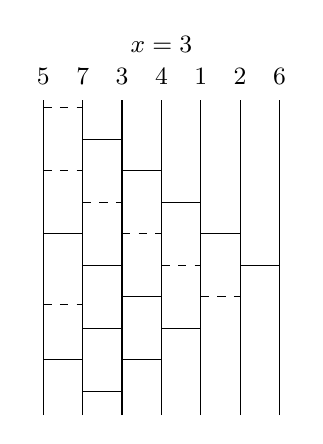
\begin{tikzpicture}
     \draw(0, 0) to (0, 4);
            \draw(0, 2.3) to (0.5, 2.3);
            \draw(0, 0.7) to (0.5, 0.7);
        \draw(.5, 0) to (.5, 4);
            \draw(.5, 1.9) to (1, 1.9);
            \draw(0.5, 1.1) to (1, 1.1);
            \draw(0.5, 0.3) to (1, 0.3);
        \draw(1, 0) to (1, 4);
            \draw(1, 1.5) to (1.5, 1.5);
            \draw(1, 0.7) to (1.5, 0.7);
        \draw(1.5, 0) to (1.5, 4);
            \draw(1.5, 1.1) to (2, 1.1);
            \draw(1.5, 2.7) to (2, 2.7);
        \draw(2, 0) to (2, 4);
        \draw(2.5, 0) to (2.5, 4);
        \draw(3, 0) to (3, 4);
       

        \draw(2.5, 1.9) to (3, 1.9);
        \draw(2.0, 2.3) to (2.5, 2.3);

        \draw(1.0, 3.1) to (1.5, 3.1);
        \draw(0.5, 3.5) to (1.0, 3.5);
      
        \draw[dashed] (0, 3.9) -- (0.5, 3.9);
        \draw[dashed] (2, 1.5) -- (2.5, 1.5);
        \draw[dashed] (1.5, 1.9) -- (2.0, 1.9);
        \draw[dashed] (1.0, 2.3) -- (1.5, 2.3);
        \draw[dashed] (0.5, 2.7) -- (1.0, 2.7);
        \draw[dashed] (0.0, 3.1) -- (0.5, 3.1);
        \draw[dashed] (0.0, 1.4) -- (0.5, 1.4);
        

        \node at(1.5, 4.7){\small{$x=3$}};
        \node at(0, 4.3){\small{$5$}};
        \node at(.5, 4.3){\small{$7$}};
        \node at(1, 4.3){\small{$3$}};
        \node at(1.5, 4.3){\small{$4$}};
        \node at(2, 4.3){\small{$1$}};
        \node at(2.5, 4.3){\small{$2$}};
        \node at(3, 4.3){\small{$6$}};
    \end{tikzpicture}
    \end{minipage}
    \begin{minipage}{.3\textwidth}
   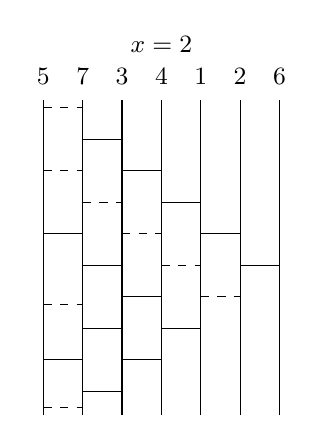
\begin{tikzpicture}
     \draw(0, 0) to (0, 4);
            \draw(0, 2.3) to (0.5, 2.3);
            \draw(0, 0.7) to (0.5, 0.7);
        \draw(.5, 0) to (.5, 4);
            \draw(.5, 1.9) to (1, 1.9);
            \draw(0.5, 1.1) to (1, 1.1);
            \draw(0.5, 0.3) to (1, 0.3);
        \draw(1, 0) to (1, 4);
            \draw(1, 1.5) to (1.5, 1.5);
            \draw(1, 0.7) to (1.5, 0.7);
        \draw(1.5, 0) to (1.5, 4);
            \draw(1.5, 1.1) to (2, 1.1);
            \draw(1.5, 2.7) to (2, 2.7);
        \draw(2, 0) to (2, 4);
        \draw(2.5, 0) to (2.5, 4);
        \draw(3, 0) to (3, 4);
      


        \draw(2.5, 1.9) to (3, 1.9);
        \draw(2.0, 2.3) to (2.5, 2.3);

        \draw(1.0, 3.1) to (1.5, 3.1);
        \draw(0.5, 3.5) to (1.0, 3.5);
      
        \draw[dashed] (0, 3.9) -- (0.5, 3.9);
        \draw[dashed] (2, 1.5) -- (2.5, 1.5);
        \draw[dashed] (1.5, 1.9) -- (2.0, 1.9);
        \draw[dashed] (1.0, 2.3) -- (1.5, 2.3);
        \draw[dashed] (0.5, 2.7) -- (1.0, 2.7);
        \draw[dashed] (0.0, 3.1) -- (0.5, 3.1);
        \draw[dashed] (0.0, 1.4) -- (0.5, 1.4);
        \draw[dashed] (0.0, 0.1) -- (0.5,0.1);
        

        \node at(1.5, 4.7){\small{$x=2$}};
        \node at(0, 4.3){\small{$5$}};
        \node at(.5, 4.3){\small{$7$}};
        \node at(1, 4.3){\small{$3$}};
        \node at(1.5, 4.3){\small{$4$}};
        \node at(2, 4.3){\small{$1$}};
        \node at(2.5, 4.3){\small{$2$}};
        \node at(3, 4.3){\small{$6$}};

    \end{tikzpicture}
    \end{minipage}
    

        
        % \node at(9.5, -5.3){\small{$x=2,row=10$}};

        % \node at(0, -.7){\small{$5$}};
        % \node at(.5, -.7){\small{$7$}};
        % \node at(1, -.7){\small{$3$}};
        % \node at(1.5, -.7){\small{$4$}};
        % \node at(2, -.7){\small{$1$}};
        % \node at(2.5, -.7){\small{$2$}};
        % \node at(3, -.7){\small{$6$}};
        
        % \node at(4, -.7){\small{$5$}};
        % \node at(4.5, -.7){\small{$7$}};
        % \node at(5, -.7){\small{$3$}};
        % \node at(5.5, -.7){\small{$4$}};
        % \node at(6, -.7){\small{$1$}};
        % \node at(6.5, -.7){\small{$2$}};
        % \node at(7, -.7){\small{$6$}};

        % \node at(8, -.7){\small{$5$}};
        % \node at(8.5, -.7){\small{$7$}};
        % \node at(9, -.7){\small{$3$}};
        % \node at(9.5, -.7){\small{$4$}};
        % \node at(10, -.7){\small{$1$}};
        % \node at(10.5, -.7){\small{$2$}};
        % \node at(11, -.7){\small{$6$}};
        
    
    \caption{The ordering of the state of the ladder when creating the root ladder for $(5,7,3,4,1,2,6)$}
    \label{Fig:CreateRoot}
\end{figure}

% \begin{lemma}
% 	The time complexity for CreateRoot is $O(n^{2})$
% \end{lemma}
% \begin{proof}
% 	The for-loop runs from some arbitrary index to $n$ on each function call. Thus, we get $O(n)$. The following 
%     recursion holds, $CreateRoot(n-k) = CreateRoot((n-k)+1) + n=CreateRoot((n-k)+2) + n-1\dots $. The recurrence 
%     relation is reduced to $n(n+1)/2= O(n^2)$.
% \end{proof}

A main contribution of this thesis is the canonical ladder and the algorithm {\sc CreateCanonical}.
By defining the canonical ladder we are able to list all $n!$ canonical ladders in any order. 
Let $L_{n}$ be the set of all $n!$ canonical ladders. 
\begin{lemma}
    Using {\sc CreateCanonical}, we can list $L_{n}$ in any order.
\end{lemma}
\begin{proof}
 Let $S_{n}$ be the set of all permutations of order $n$. We simply apply an ordering to list $S_{n}$. For each 
 permutation in $S_{n}$, we apply {\sc CreateCanonical}, thus listing $L_{n}$ in the same order as $S_{n}$.
\end{proof}
We create each $CL(\pi)$ in $O(n^2)$ time using {\sc CreateCanonical}. However, using {\sc CreateCanonical} to list $L_{n}$ is inefficient, 
seeing as each ladder is created in $O(n^2)$ time. 
In chapters 4 and 5 we provide two Gray code listing algorithms, {\sc ModifiedSJT} and {\sc ListLnByKBars}, to list $L_{n}$ in constant amortized time. 
The details of these algorithms are found in chapters 4 and 5 respectively.  
% {\sc ModifiedSJT} and {\sc CyclicBar} require additional auxiliary functions. We define {\sc Inv(x)} as follows: $|\forall y \in \pi : y < x, p_{y}>p_{x}|$. 
% For example, given $(3,4,1,5,6,2)$, {\sc Inv(1)=0}, {\sc Inv(2)=0}, {\sc Inv(3)=2}, {\sc Inv(4)=2}, {\sc Inv(5)=1}, {\sc Inv(6)=1}. 
% Given {\sc Inv(x)}, 
% we can define the function {\sc GetCoordinates2}. In order to define {\sc GetCoordinates2}, let $x>y \in \pi$. Given 
% $p_{x}$ and $p_{y}$, suppose a transposition were applied to $x$ and $y$. Prior to the transposition 
% of $x$ and $y$, if $p_{x} = p_{y}-1$ then {\sc GetCoordinates2} returns the row and column of the bar $(x,y)$ to be removed 
% from the ladder. If $p_{x}=p_{y}+1$, then {\sc GetCoordinates} returns 
% the row and column of bar $(x,y)$ to be added to the ladder. 





